%% LSST efforts for dark sirens
\textbf{Dark Siren Measurements for Precision Cosmology:}
I will pursue a cutting-edge program that creates a gold-standard photometric galaxy catalog for dark siren cosmology using \LSST\ data.
% LSST DP2 characterization in prep for DR1
This program is structured in four stages, structured around forthcoming data releases (see Figure~\ref{fig:imaging_surveys}), each building towards a powerful, world leading measurement.

This begins with an ongoing project, focused on characterizing the \LSST\ Data Preview 2 (DP2) galaxy catalog, aiming to define robust and scalable object classification for future \LSST\ data releases.
% DESC Y1 forecasting
Following characterization of DP2, I will finish a forecasting study that quantifies the $H_0$ precision achievable by combining simulated first-year LSST data with an O4-like gravitational-wave catalog, extending the dark-siren methodology from my recent \DELVE\ measurement to project the constraining power in the \LSST\ era.
% LSST DR1 measurement
Superceding DP2 preparation, I will characterize the first \LSST\ Data Release (DR1) galaxy catalog and produce a dark siren measurement of $H_0$. This result will extend the 
methodology I developed with \DELVE\ to a dataset with substantially greater depth, area, and photometric 
\begin{wrapfigure}{l}{0.5\textwidth}
    \centering
    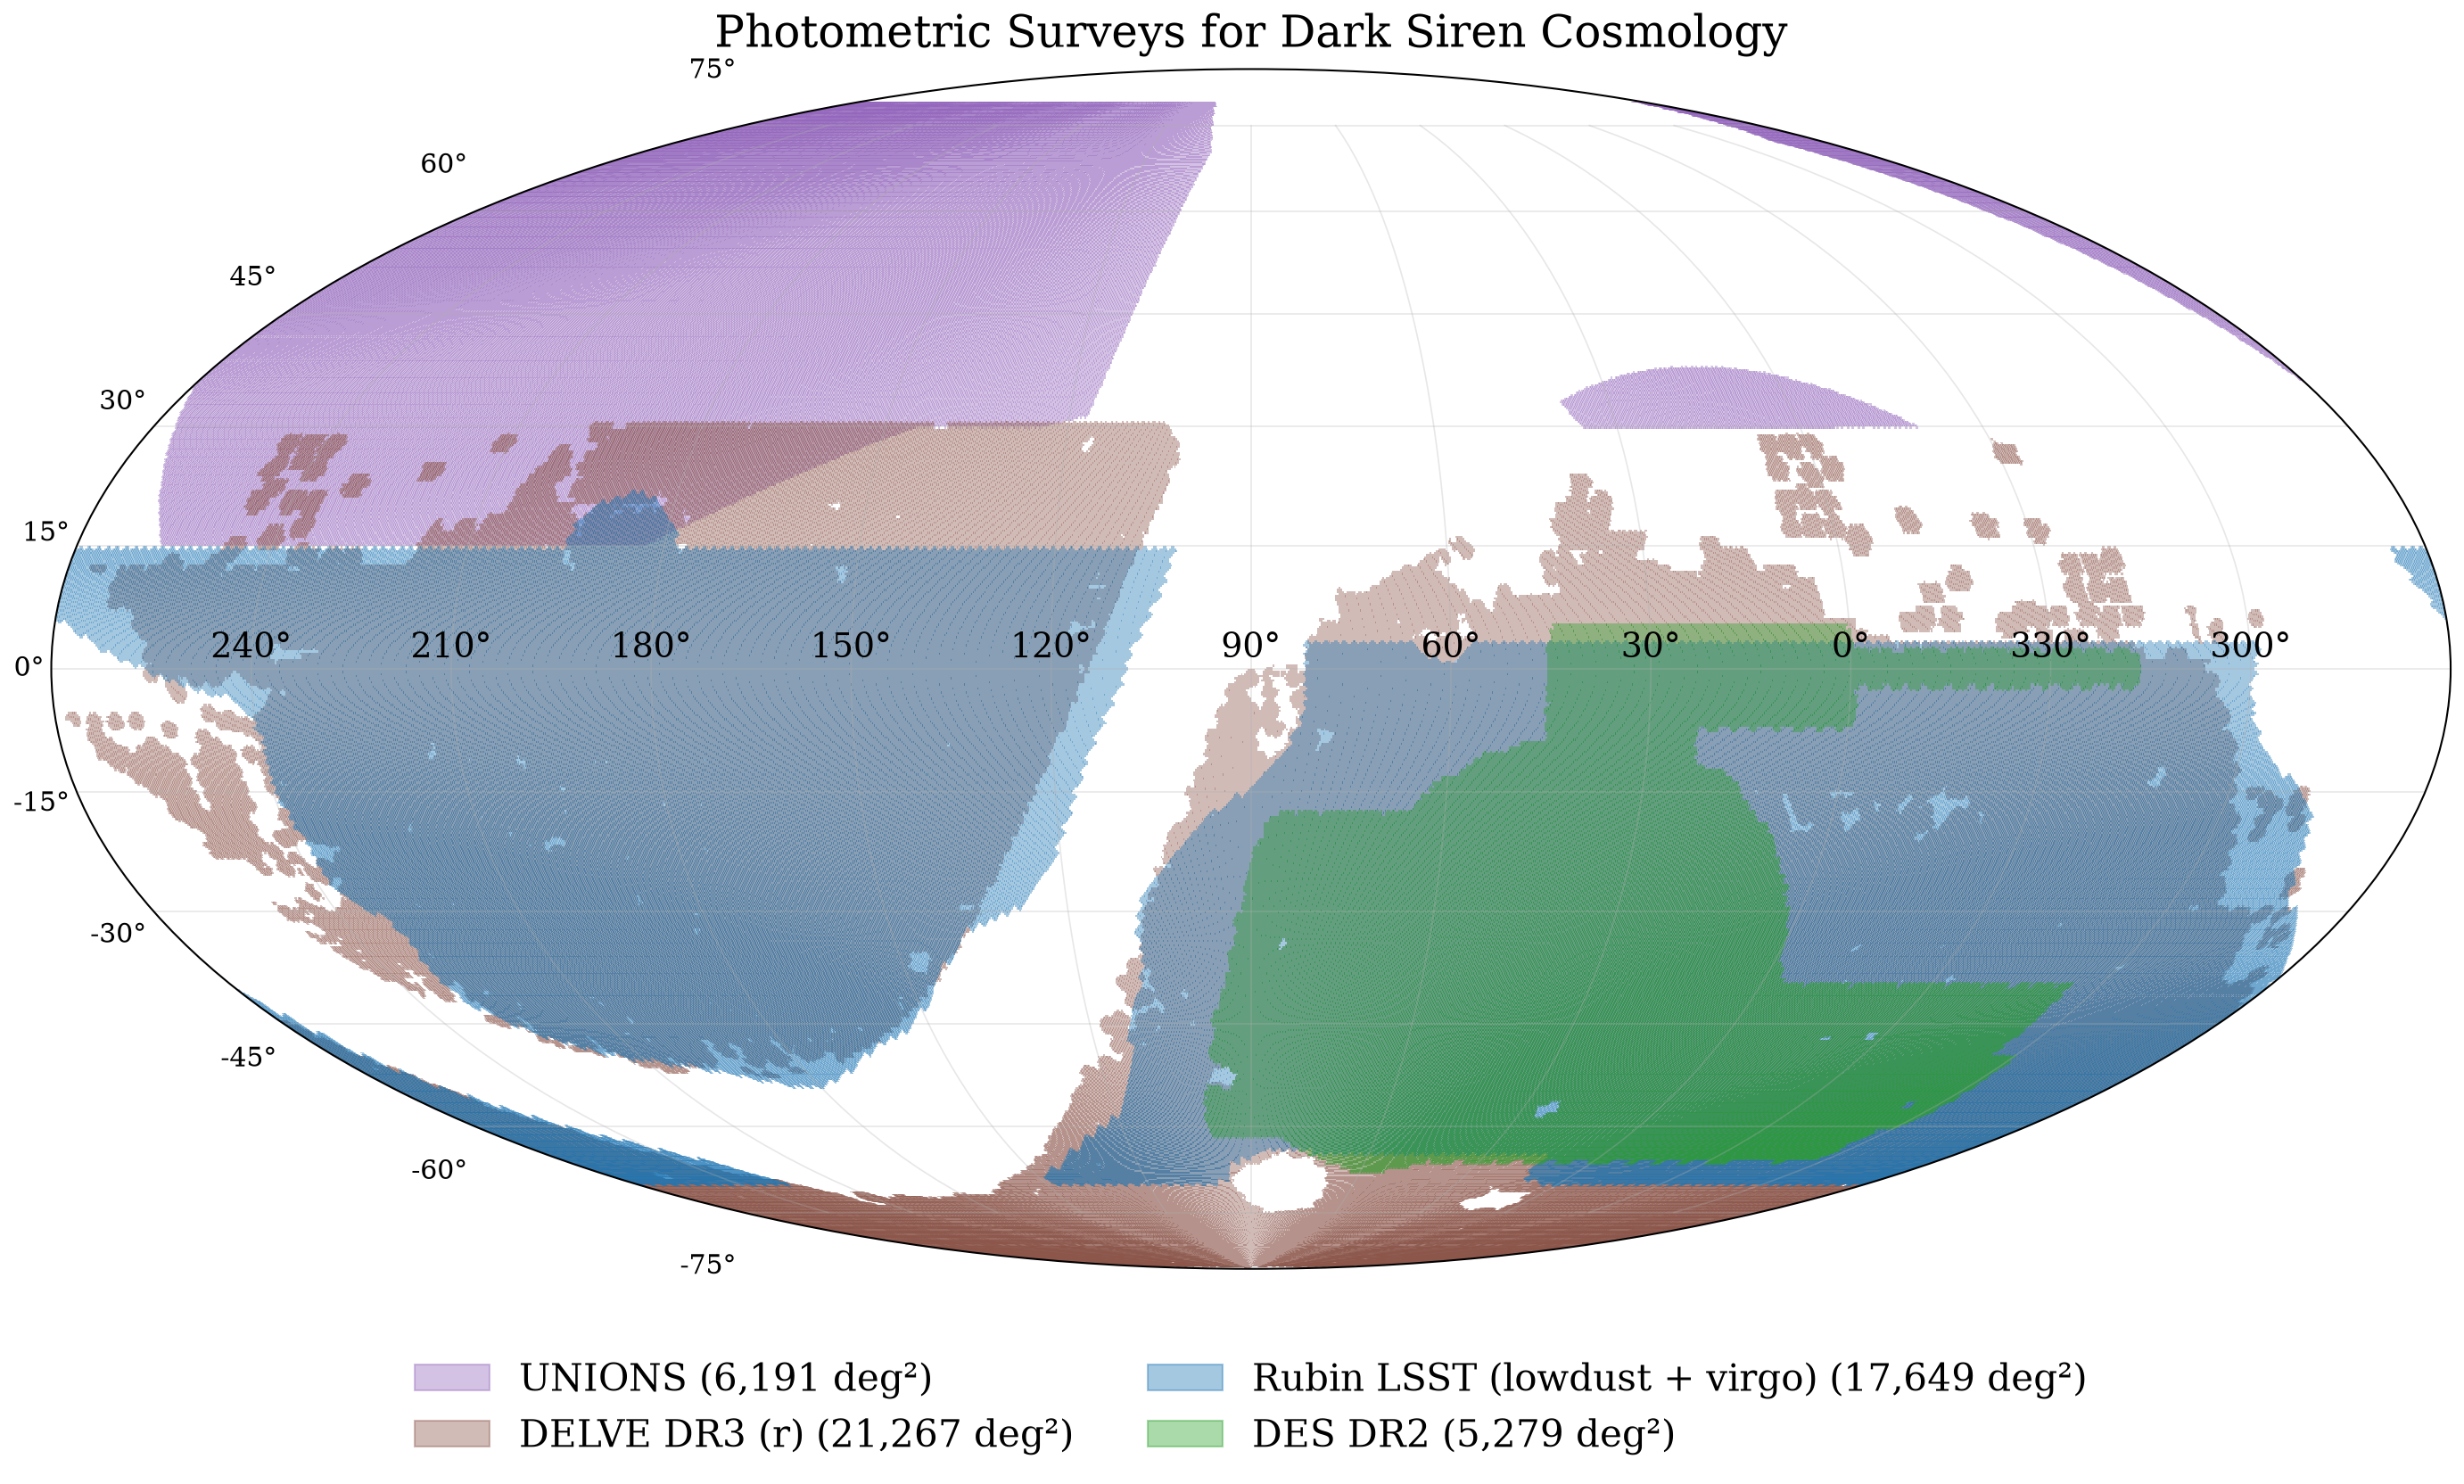
\includegraphics[width=\linewidth]{specific_positions/AY26/cfa_prize_fellowship/research_statement/figures/image.png}
    \caption{Sky coverage of the photometric galaxy surveys used for dark siren cosmology: UNIONS (6,191 $\deg^2$, purple), Rubin LSST (low-dust and Virgo footprint, 17,649 $\deg^2$, blue), DES DR2 (5,279 $\deg^2$, green), and DELVE (21,267 $\deg^2$, brown). UNIONS covers the northern sky that DES, DELVE and LSST cannot reach. The southern surveys overlap substantially, so a catalog comprised of the best available photometry in any sky region can span a large fraction of the extragalactic sky.}
    \label{fig:imaging_surveys}
\end{wrapfigure}
uniformity, all features that will make it the standard galaxy catalog for dark siren analyses.
% LSST DR1 combined probes - emphasize shear instead of clustering
Building on the DR1 measurement, I aim to combine \LSST\ large-scale structure measurements in a joint cosmological analysis, using cosmic shear and standard sirens to obtain a tighter constraint of $H_0$, and extend the constraints to $\Omega_m$.
%% Adapting other data for Dark sirens, either through specialized surveys, or through existing data
% GWCats - mention when discussing the existing collaboration for GW-Primo

As the wealth of \GW\ data increases alongside a wide variety of new galaxy catalog data, I will explore the frontier of the standard siren method using specialized observational programs and forthcoming data releases from other surveys,
%and a rigorous assessment of systematics for standard sirens,
while engaging with the Horizon Europe-funded GWCats collaboration, a tight-knit group of researchers focused on using galaxy catalogs and \GW\ data to constrain cosmology.
% NORTHSTARS
To assess the frontier of the dark siren method using observations, I will lead a dedicated spectroscopic dark-siren pilot survey, obtaining targeted redshifts within GW localization volumes to assess the limits and enhancements to $H_0$ constraints using well-localized dark sirens. This survey is led through a continuing collaboration with \JGEM\ on the \PFS\ instrument, obtaining additional observations for the GW merger pursued in our collaborative \DESGW\ \ToO\, with an expected observation date starting in April 2027 (see Figure~\ref{fig:pfs_coverage}).
% GW-primo
In parallel, I am leading the image processing for a similar survey, the Gravitational Wave Photometric Redshift Improvement with Medium-band Observations (GW-Primo) project, to test how medium band observations improve $H_0$ precision through enhanced photometric redshifts. By comparing the results of these two survey programs, I will be able to assess which route, enhanced photometric or spectroscopic, will provide the best constraints on $H_0$ given limited telescope time and the current sample of GWs.

% UNIONS
Similar to \DES\ and \LSST, the \UNIONS\ survey provides a large area galaxy catalog in the Northern hemisphere, where \DES\ and \LSST\ coverage is not possible. I will prepare the  \UNIONS\ galaxy catalog for dark siren cosmology through ongoing work with the \UNIONS\ collaboration, applying the lessons from the \DELVE\ galaxy catalog preparation. I will construct both an isolated \UNIONS\ catalog and a combined galaxy catalog of \UNIONS\ and \LSST\ data for standard siren cosmology, while taking care to control any systematics that come from joining different galaxy catalogs. This combined catalog will span a large portion of the extragalactic sky (see Figure~\ref{fig:imaging_surveys}), including several well localized GWs in the northern hemisphere, all with comparable photometric redshift quality to the \LSST\ due to the addition of u-band photometry. In all, this joint catalog will be a value-added catalog compared to \LSST\ data alone, not limited to augmenting dark siren cosmology.

% PV methodological study
% Finally, with the new discovery capabilities of \Rubin\ for bright standard sirens, the systematics of multiple bright siren measurements must be thoroughly examined before claiming a robus and precise measurement of $H_0$. To build this foundation, I will lead an assessment of peculiar velocity systematics in bright siren measurements, using synthetic and real data to accurately map the velocity field and reduce the systematic contribution to future bright siren measurements.
